\documentclass{report}
\usepackage[spanish]{babel}
\usepackage[utf8]{inputenc}
\usepackage{graphicx, longtable, float, titlesec, hyperref, enumitem, dingbat, soul, multicol, listings}
\usepackage[dvipsnames]{xcolor}
\usepackage[margin=2cm]{geometry}

% Cambia el color de los links
\hypersetup{hidelinks}

% Generamos un comando para saltar pagina con las secciones
\NewDocumentCommand{\cpsection}{s o m}{%
  \clearpage
  \IfBooleanTF{#1}
    {\section*{#3}}
    {%
      \IfNoValueTF{#2}
        {\section{#3}}
        {\section[#2]{#3}}%
    }%
}

% Python Code
\lstdefinestyle{Python}{
  commentstyle=\color{brown},
  keywordstyle=\color{violet},
  numberstyle=\tiny\color{gray},
  stringstyle=\color{purple},
  basicstyle=\ttfamily\footnotesize,
  breakatwhitespace=false,         
  breaklines=true,                 
  captionpos=b,                    
  keepspaces=true,                 
  numbers=left,                    
  numbersep=5pt,                  
  showspaces=false,                
  showstringspaces=false,
  showtabs=false,                  
  tabsize=2,
  literate={ñ}{{\~n}}1 {á}{{\'a}}1 {é}{{\'e}}1 {í}{{\'i}}1 {ó}{{\'o}}1 {ú}{{\'u}}1
}
\lstset{style=Python}

% Elimina la palabra "Capítulo" de los títulos de los capítulos
\titleformat{\chapter}[display]
  {\normalfont\bfseries}{}{0pt}{\Huge\thechapter.\space}

\titleformat{name=\chapter,numberless}[display]
  {\normalfont\bfseries}{}{0pt}{\Huge}

\titlespacing*{\chapter}{0pt}{-50pt}{20pt}

% Personalización del índice de listados
\renewcommand{\lstlistingname}{Código}  % Cambiar el nombre de "Listing" a "Código"
\renewcommand{\lstlistlistingname}{Índice de Códigos}

% Añade numeración a los subsubsection*s y los añade al índice
\setcounter{secnumdepth}{4}
\setcounter{tocdepth}{4}

\begin{document}
  \begin{titlepage}
      \centering
      
\includegraphics[width=0.6\textwidth]{./.img/logo.jpg}\\
      \vspace{1cm}
      \LARGE Técnicas de Inteligencia Artificial\\
      \vspace{0.5cm}
      \Large Ingeniería Informática de Gestión y Sistemas de Información\\
      \vspace{3cm}
      \Huge Practica 3\\
      \huge Clasificacion\\
      \vspace{2.5cm}
      \Large Autor(es):\\
      \vspace{0.2cm}
      \large Xabier Gabiña\\
      \large Diego Montoya\\
      \vfill
      \today
  \end{titlepage}
  \tableofcontents
  \listoffigures
  %\listoftables
  \lstlistoflistings
  \chapter{Introducción}
    \paragraph*{}
    {
      En esta práctica de laboratorio exploramos diversas técnicas de aprendizaje automático aplicadas a problemas de regresión y clasificación, con un enfoque particular en la implementación y optimización de modelos basados en redes neuronales. La práctica se divide en tres ejercicios principales, cada uno de los cuales aborda un problema específico: la regresión no lineal, la clasificación de dígitos y la clasificación de sentimientos.\\

      El objetivo principal es aplicar conceptos fundamentales de aprendizaje profundo, incluyendo el uso de funciones de activación como ReLU, técnicas de optimización como descenso de gradiente, y métodos para evitar el sobreajuste, tales como regularización, dropout y early stopping. Adicionalmente, se busca comparar los resultados obtenidos y evaluar el desempeño de los modelos implementados en términos de métricas como la pérdida y la precisión.\\

      En el primer ejercicio, se desarrolla un modelo de regresión no lineal utilizando redes neuronales con el objetivo de aproximar una función no lineal dada. En el segundo ejercicio, se aborda la clasificación de imágenes de dígitos manuscritos utilizando el conjunto de datos MNIST, lo que permite explorar tareas de clasificación multiclase. Finalmente, en el tercer ejercicio, se diseña y optimiza un modelo para la clasificación de sentimientos, incorporando técnicas avanzadas para mejorar la generalización del modelo.\\

      A lo largo de esta práctica, se realiza un análisis detallado del impacto de los hiperparámetros y de las técnicas implementadas, permitiendo así una comprensión profunda de los fundamentos del aprendizaje automático y su aplicación práctica en diferentes dominios.\\
    }
  \chapter{Ejercicios}
    \section{Regresión no lineal}
      \subsection*{Descripción}
        \paragraph*{}
        {
          La regresión no lineal se utiliza para encontrar relaciones entre variables cuando estas no son lineales.
          La principal diferencia con la regresión lineal es que no se ajusta una recta a los datos.
          Lo que se hace es utilizar una curva (exponencial, logarítmica o polinómica) para ajustar los datos y encontrar la relación entre las variables.
          \begin{figure}[H]
            \centering
            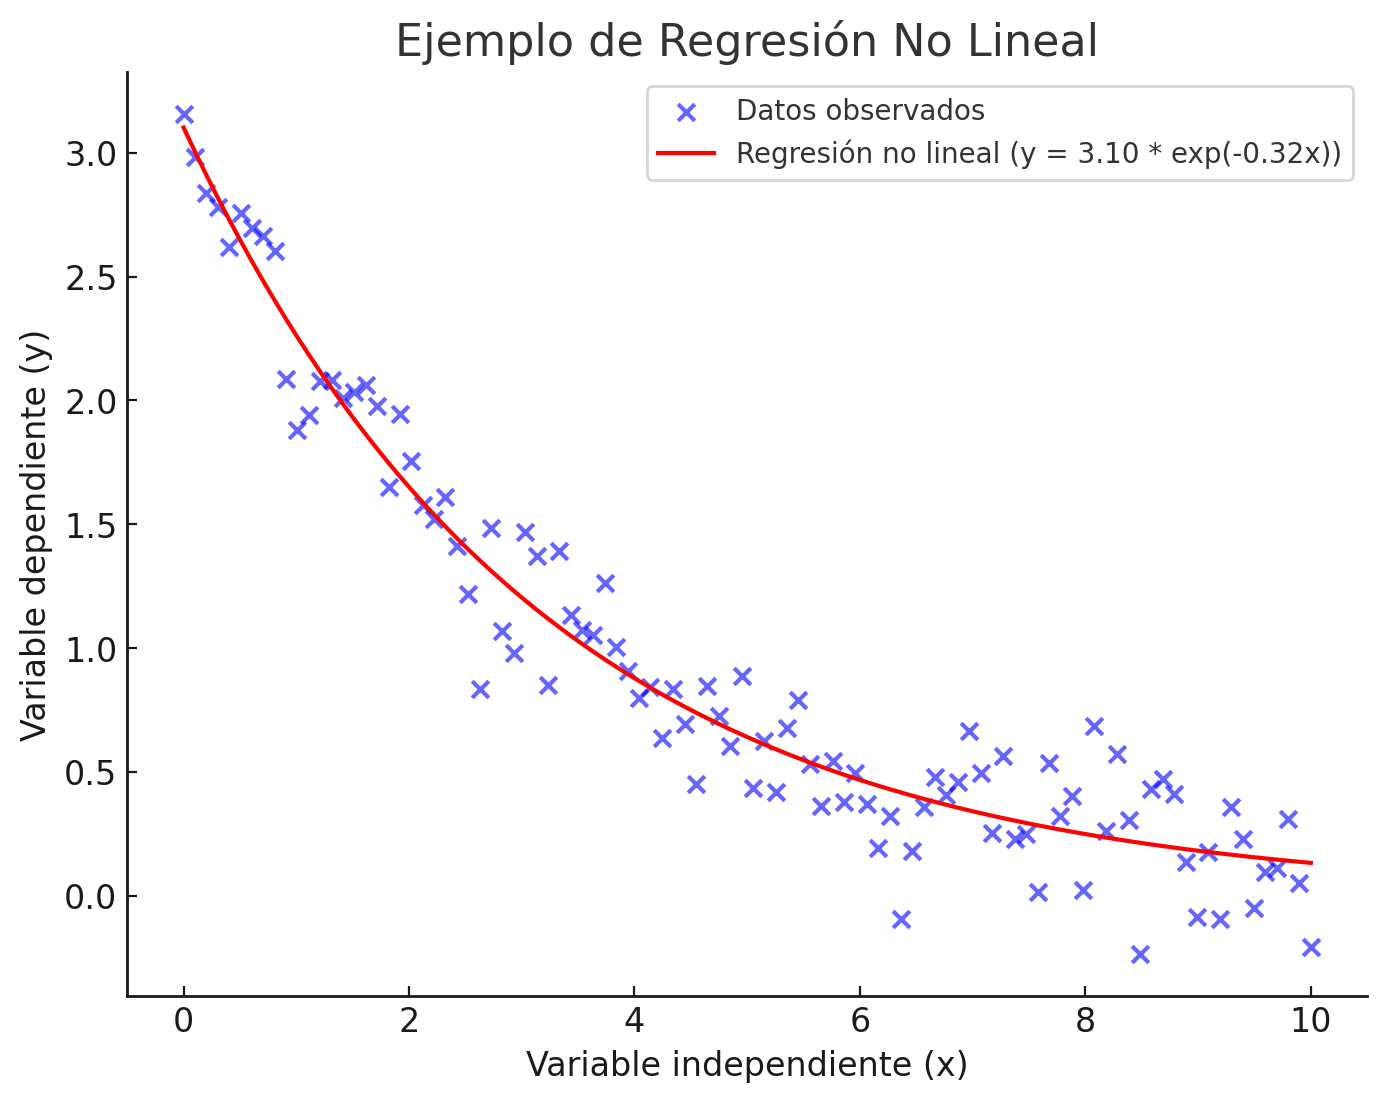
\includegraphics[width=0.5\textwidth]{.img/rnl.png}
            \caption{Ejemplo de regresión no lineal}
          \end{figure}
        }
      \subsection*{Implementación}
        \begin{lstlisting}[language=Python, caption=Implementación de la regresión no lineal]
class RegressionModel(object):
  """
  A neural network model for approximating a function that maps from real
  numbers to real numbers. The network should be sufficiently large to be able
  to approximate sin(x) on the interval [-2pi, 2pi] to reasonable precision.
  NO ES CLASIFICACION, ES REGRESION. ES DECIR; APRENDER UNA FUNCION.
  SI ME DAN X TENGO QUE APRENDER A OBTENER LA MISMA Y QUE EN LA FUNCION ORIGINAL DE LA QUE QUIERO APRENDER
  """
  def __init__(self):
      # Tamaño del batch
      self.batch_size = 4
      # Layer 0
      self.w0 = nn.Parameter(1, 10)
      self.b0 = nn.Parameter(1, 10)
      # Layer 1
      self.w1 = nn.Parameter(10, 10)
      self.b1 = nn.Parameter(1, 10)
      # Layer 2
      self.w2 = nn.Parameter(10, 10)
      self.b2 = nn.Parameter(1, 10)
      # Layer 3
      self.w3 = nn.Parameter(10, 1)
      self.b3 = nn.Parameter(1, 1)
      # Learning rate
      self.lr = -0.005
      
  def run(self, x):
      """
      Runs the model for a batch of examples.

      Inputs:
          x: a node with shape (batch_size x 1). En este caso cada ejemplo solo esta compuesto por un rasgo
      Returns:
          A node with shape (batch_size x 1) containing predicted y-values.
          Como es un modelo de regresion, cada valor y tambien tendra un unico valor
      """
      layer0 = nn.ReLU(nn.AddBias(nn.Linear(x, self.w0), self.b0))
      layer1 = nn.ReLU(nn.AddBias(nn.Linear(layer0, self.w1), self.b1))
      layer2 = nn.ReLU(nn.AddBias(nn.Linear(layer1, self.w2), self.b2))
      return nn.AddBias(nn.Linear(layer2, self.w3), self.b3)
      
  def get_loss(self, x, y):
      """
      Computes the loss for a batch of examples.

      Inputs:
          x: a node with shape (batch_size x 1)
          y: a node with shape (batch_size x 1), containing the true y-values
              to be used for training
      Returns: a loss node
              ----> ES FACIL COPIA Y PEGA ESTO Y ANNADE LA VARIABLE QUE HACE FALTA PARA CALCULAR EL ERROR 
              return nn.SquareLoss(self.run(x),ANNADE LA VARIABLE QUE ES NECESARIA AQUI), para medir el error, necesitas comparar el resultado de tu prediccion con .... que?
      """
      return nn.SquareLoss(self.run(x), y)

  def train(self, dataset):
      """
      Trains the model.
      
      """
      
      batch_size = self.batch_size
      while True:
          total_loss = 0
          for x, y in dataset.iterate_once(batch_size):
              loss = self.get_loss(x, y)
              total_loss = nn.as_scalar(loss)
              grad_wrt_w0, grad_wrt_b0, grad_wrt_w1, grad_wrt_b1, grad_wrt_w2, grad_wrt_b2, grad_wrt_w3, grad_wrt_b3 = nn.gradients(loss, [self.w0, self.b0, self.w1, self.b1, self.w2, self.b2, self.w3, self.b3])
              self.w0.update(grad_wrt_w0, self.lr)
              self.b0.update(grad_wrt_b0, self.lr)
              self.w1.update(grad_wrt_w1, self.lr)
              self.b1.update(grad_wrt_b1, self.lr)
              self.w2.update(grad_wrt_w2, self.lr)
              self.b2.update(grad_wrt_b2, self.lr)
              self.w3.update(grad_wrt_w3, self.lr)
              self.b3.update(grad_wrt_b3, self.lr)
          
          if total_loss < 0.02:
              break
      
        \end{lstlisting}
        \clearpage
      \subsection*{Conclusines}
        \paragraph*{}
        {
          Para implementar la regresión no lineal, hemos utilizado una red neuroanl con tres capas.
          Hemos probado con diferentes numero tanto de capas como de neuronas por capas y aunque no hemos hecho un barrido de parametros al uso, si que hemos visto que añadir más capas o neuronas de las que tenemos no mejoraban los resultados obtenidos.
          Lo que si ha marcado una diferencia ha sido el batch size y el learning rate. Al reducir el batch size la actualizacion de los pesos y sesgos se hace más frecuente y por lo tanto, el error disminuye más rapidamente. Combinando esto con un learning rate adecuado, hemos conseguido que el error final sea menor que 0.02.\\

          Tambien creemos importante mencionar el uso de ReLU.
          ReLU o Rectified Linear Unit es la funcion de activacion que nos permite que la red aprenda de manera no lineal.
          Basicamente, lo que hace es que si el valor de la neurona es negativo, lo pone a 0 y si es positivo, lo deja igual.
          
          \begin{figure}[H]
            \centering
            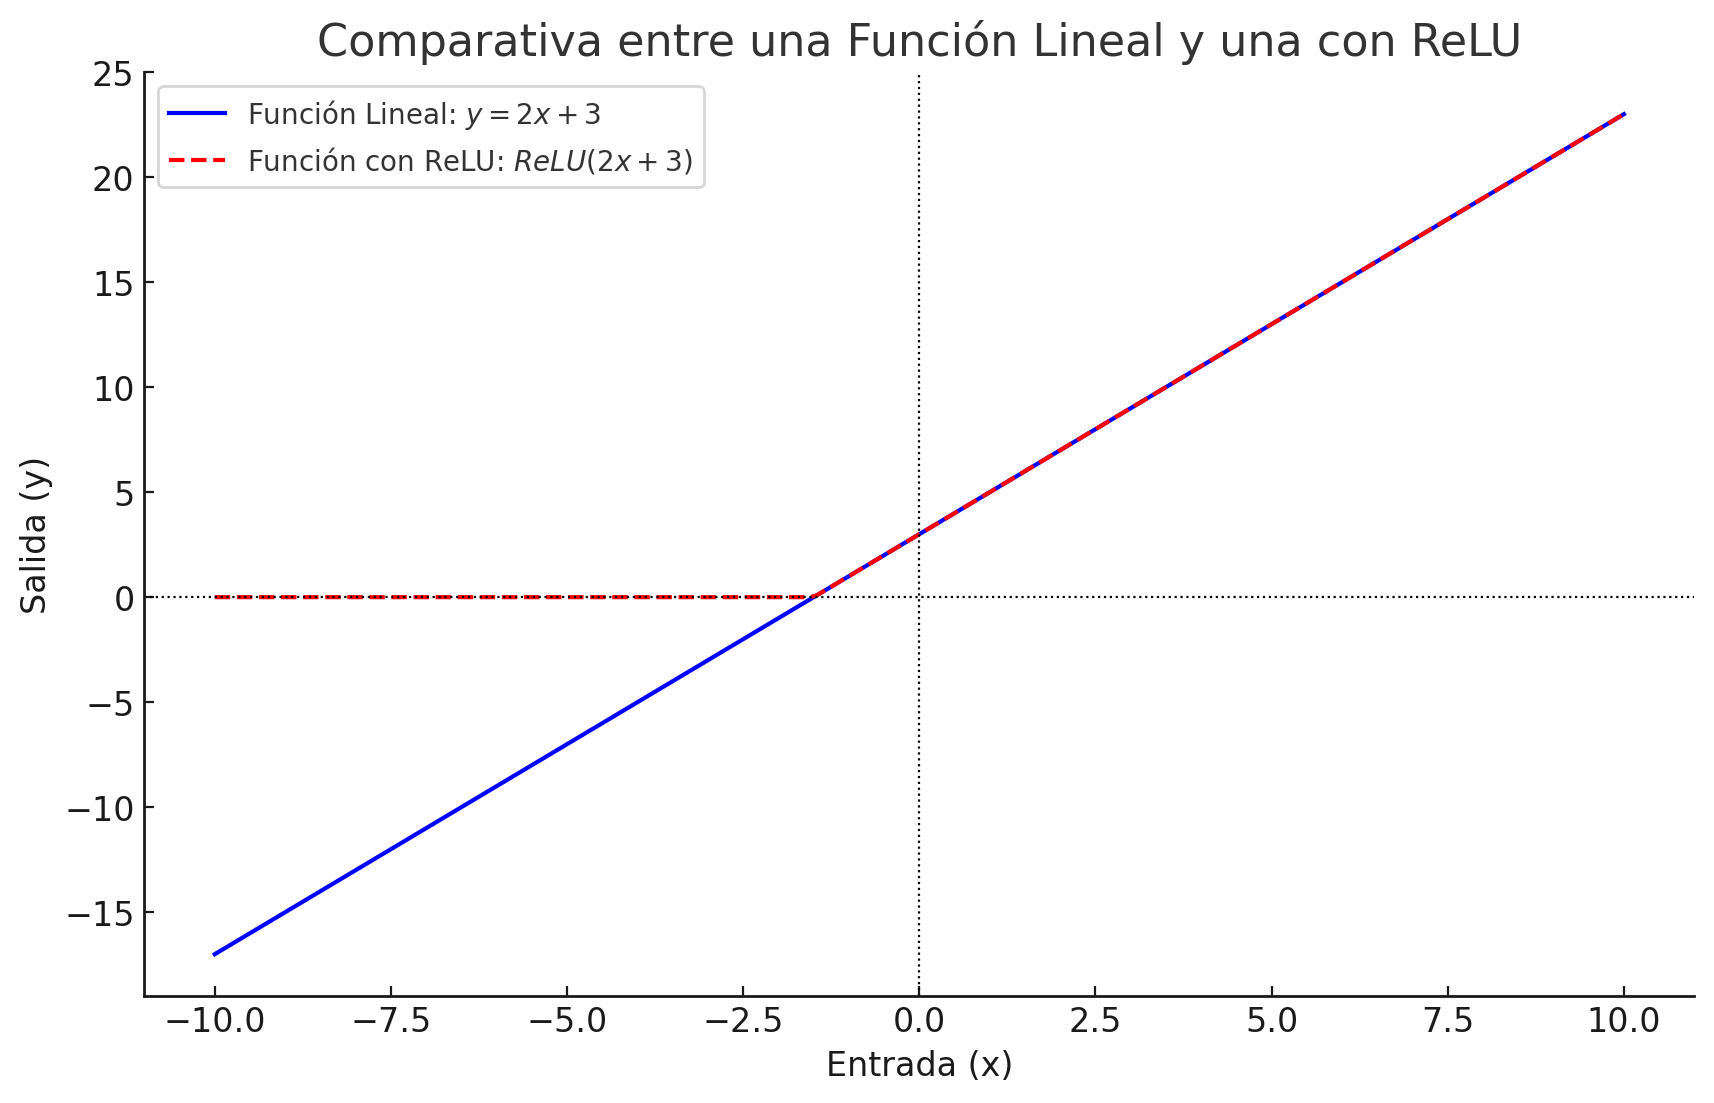
\includegraphics[width=0.5\textwidth]{.img/relu.png}
            \caption{Función de activación ReLU}
          \end{figure}

          Es posible añadir un termino de desplazamiento o punto de corte (c) para que la función no tome el valor 0 como el comienzo a tener un impacto no nulo.
          Ademas, podemos sumar una funcion al resultado de la ReLU para que a partir del punto de corte, se produzca un cambio en la pendiente en vez de generar el impacto nulo de los otros casos.
          
          \begin{figure}[H]
            \centering
            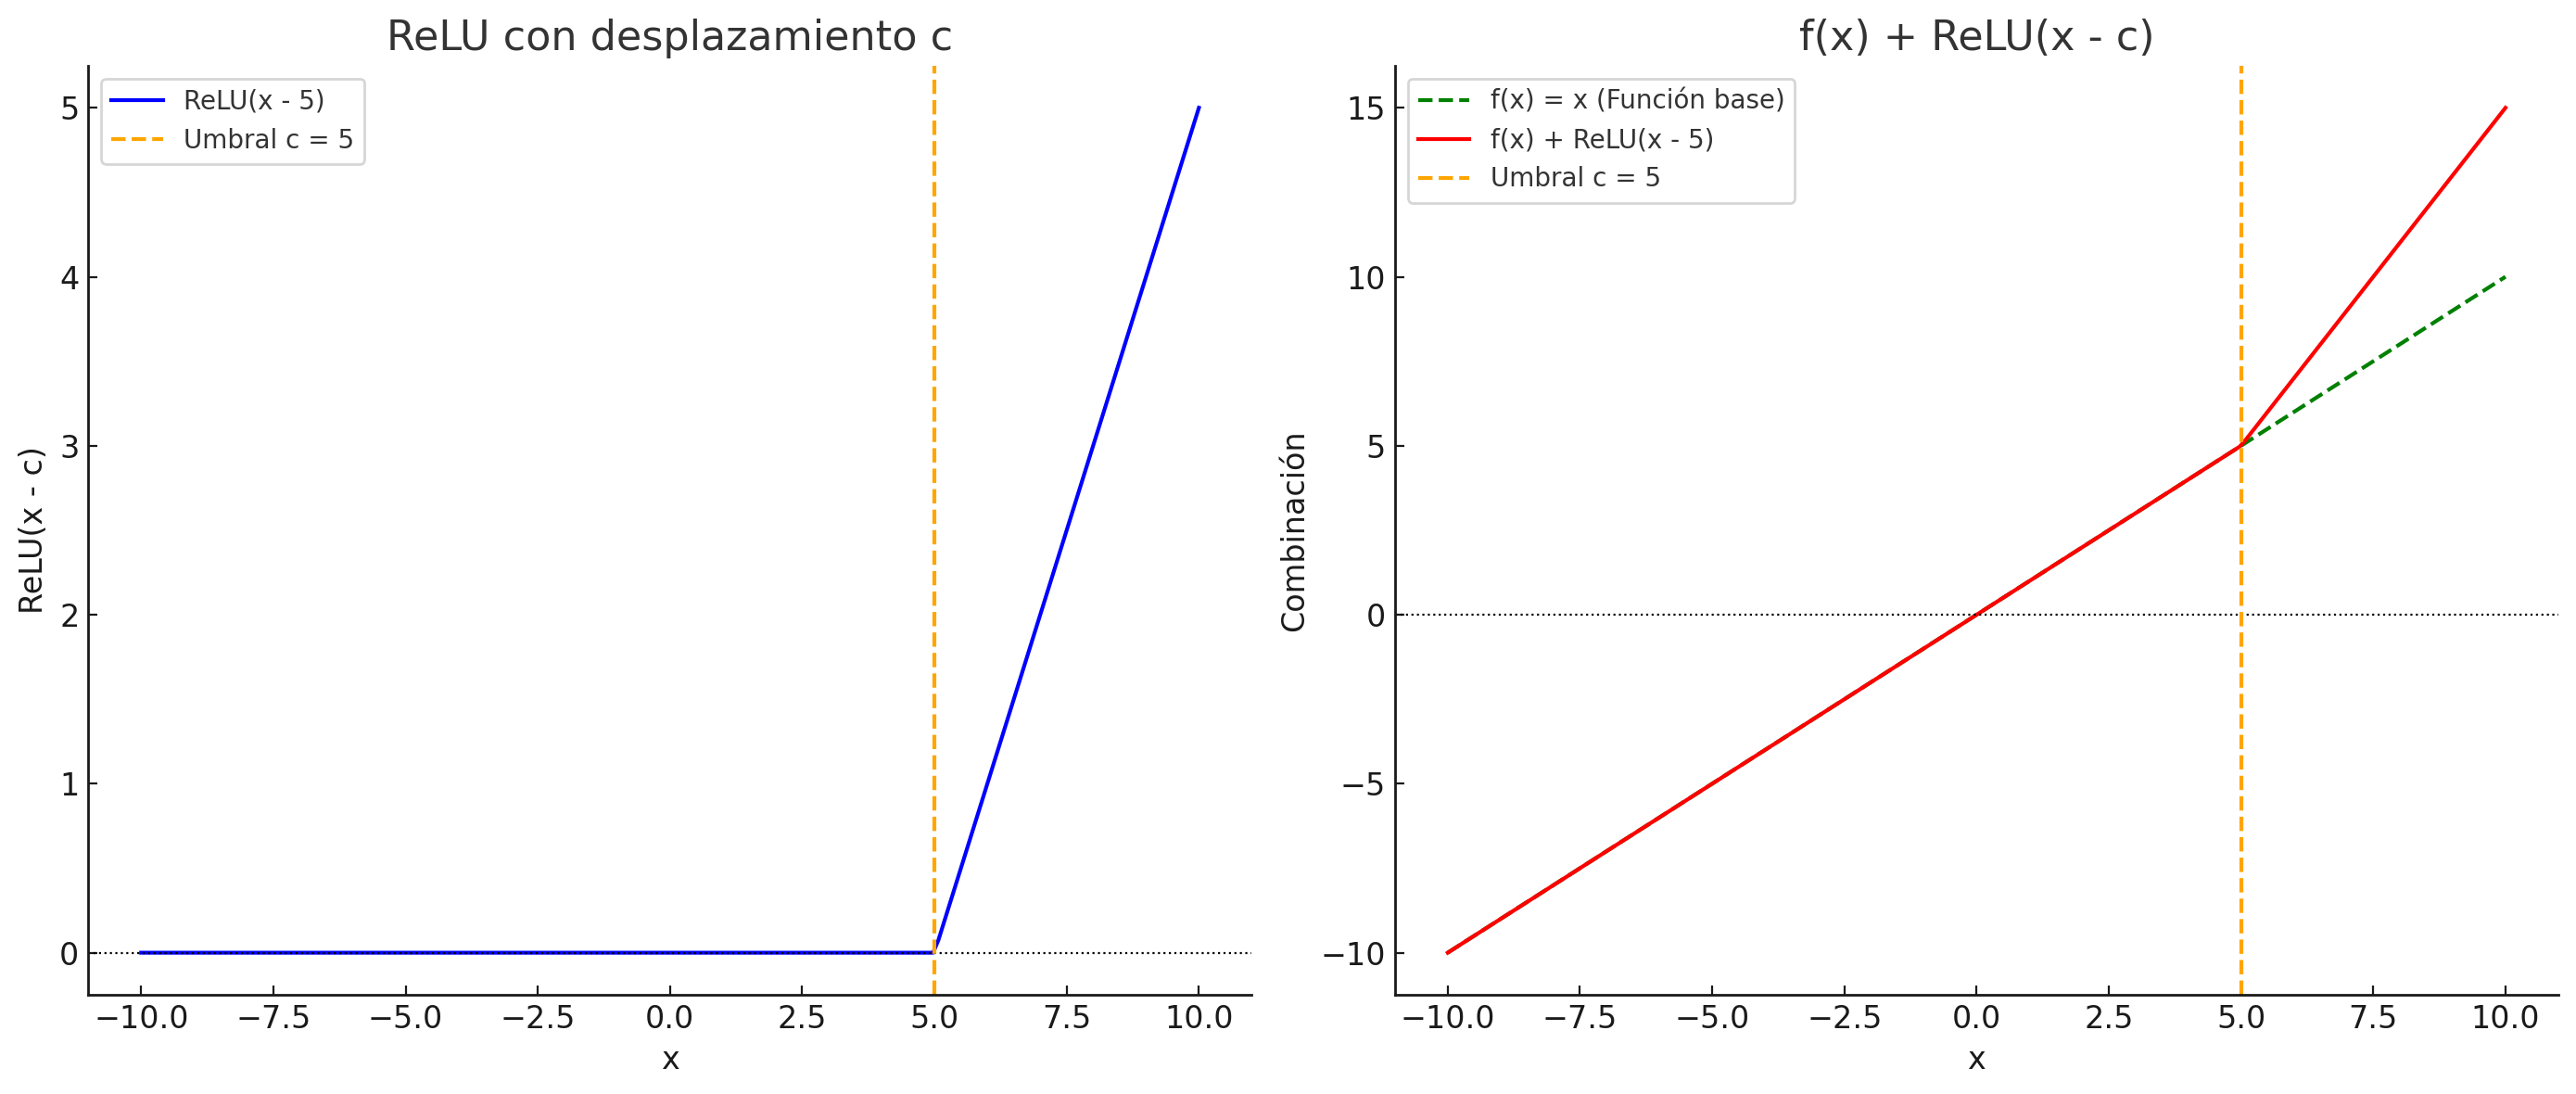
\includegraphics[width=0.9\textwidth]{.img/relu2.png}
            \caption{Función de activación ReLU con punto de corte}
          \end{figure}

          \textbf{Nota:} En algunas ejecuciones, el error final ha sido menor que 0.02, pero en otras ha sido mayor. No obstante la mayoria de las veces el resultado es positivo. Esto se debe a la aleatoriedad de los datos de entrada.
        }
    \cpsection{Clasificación de dígitos}
      \subsection*{Descripción}
        \paragraph*{}
        {
          La clasificación de dígitos es un problema de clasificación en el que se intenta clasificar un conjunto de dígitos en 10 clases (0-9).
          Para ello, se utiliza el dataset MNIST, que contiene imagenes de 28x28 píxeles y en escala de grises.
          
          \begin{figure}[H]
            \centering
            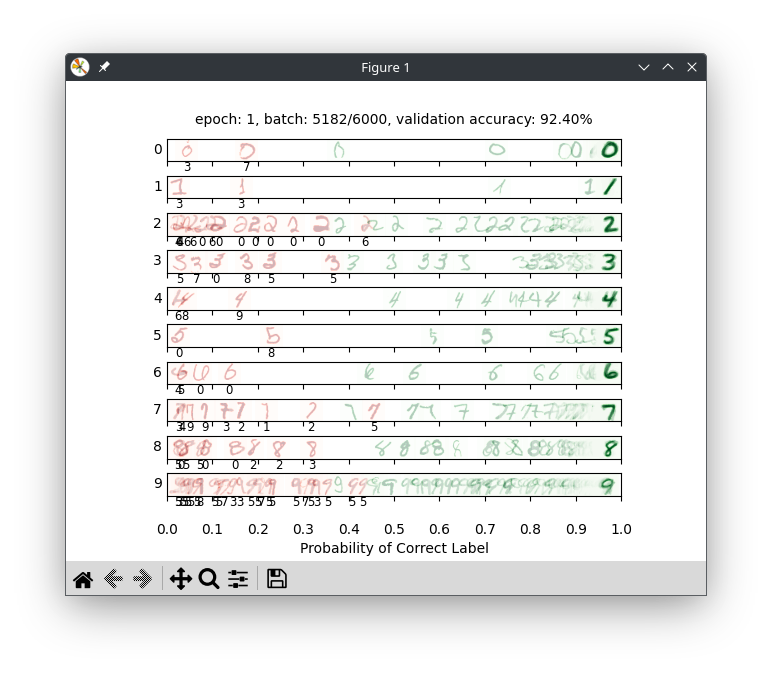
\includegraphics[width=0.8\textwidth]{.img/mnist.png}
            \caption{Ejemplo de imagen del dataset MNIST}
          \end{figure}
        }
      \subsection*{Implementación}
        \begin{lstlisting}[language=Python, caption=Implementación de la clasificación de dígitos]
class DigitClassificationModel(object):
  """
  A model for handwritten digit classification using the MNIST dataset.

  Each handwritten digit is a 28x28 pixel grayscale image, which is flattened
  into a 784-dimensional vector for the purposes of this model. Each entry in
  the vector is a floating point number between 0 and 1.

  The goal is to sort each digit into one of 10 classes (number 0 through 9).

  (See RegressionModel for more information about the APIs of different
  methods here. We recommend that you implement the RegressionModel before
  working on this part of the project.)
  """
  def __init__(self):
      # Initialize your model parameters here
      # TEN ENCUENTA QUE TIENES 10 CLASES, ASI QUE LA ULTIMA CAPA TENDRA UNA SALIDA DE 10 VALORES,
      # UN VALOR POR CADA CLASE

      # Tamaño del batch
      self.batch_size = 10
      
      # Learning rate
      self.lr = -0.1

      # Tamaño de salida
      output_size = 10
      
      # Dimensiones de la imagen
      pixel_vector_length = 28 * 28

      # Inicializa los pesos y sesgos
      # Layer 0
      self.w0 = nn.Parameter(pixel_vector_length, 100)
      self.b0 = nn.Parameter(1, 100)
      # Layer 1
      self.w1 = nn.Parameter(100, 100)
      self.b1 = nn.Parameter(1, 100)
      # Layer 2
      self.w2 = nn.Parameter(100, 100)
      self.b2 = nn.Parameter(1, 100)
      # Layer 3
      self.w3 = nn.Parameter(100, 100)
      self.b3 = nn.Parameter(1, 100)
      # Layer 4
      self.w4 = nn.Parameter(100, output_size)
      self.b4 = nn.Parameter(1, output_size)

  def run(self, x):
      """
      Corre el modelo para un lote de ejemplos.
      
      Inputs:
          x: un nodo con forma (batch_size x 784)
      Returns:
          Un nodo con forma (batch_size x 10) que contiene los valores predichos de y.
      """
      layer0 = nn.ReLU(nn.AddBias(nn.Linear(x, self.w0), self.b0))
      layer1 = nn.ReLU(nn.AddBias(nn.Linear(layer0, self.w1), self.b1))
      layer2 = nn.ReLU(nn.AddBias(nn.Linear(layer1, self.w2), self.b2))
      layer3 = nn.ReLU(nn.AddBias(nn.Linear(layer2, self.w3), self.b3))
      return nn.AddBias(nn.Linear(layer3, self.w4), self.b4)

  def get_loss(self, x, y):
      """
      Calcula la pérdida para un lote de ejemplos.
      
      Inputs:
          x: un nodo con forma (batch_size x 784) que se mete en la red para obtener las predicciones.
          y: un nodo con forma (batch_size x 10), que contiene los verdaderos valores y que se utilizarán para el entrenamiento.
      Returns: un nodo de pérdida
      """
      return nn.SoftmaxLoss(self.run(x), y) 
  
  def train(self, dataset):
      """
      Trains the model.
      EN ESTE CASO EN VEZ DE PARAR CUANDO EL ERROR SEA MENOR QUE UN VALOR O NO HAYA ERROR (CONVERGENCIA),
      SE PUEDE HACER ALGO SIMILAR QUE ES EN NUMERO DE ACIERTOS. EL VALIDATION ACCURACY
      NO LO TENEIS QUE IMPLEMENTAR, PERO SABED QUE EMPLEA EL RESULTADO DEL SOFTMAX PARA CALCULAR
      EL NUM DE EJEMPLOS DEL TRAIN QUE SE HAN CLASIFICADO CORRECTAMENTE 
      """
      while dataset.get_validation_accuracy() < 0.975:
          # Iterar sobre el dataset en lotes.
          for x, y in dataset.iterate_once(self.batch_size):
              # Calcula la pérdida.
              loss = self.get_loss(x, y)

              # Calcula el gradiente de los pesos y sesgos con respecto a la pérdida.
              gradients = nn.gradients(loss, [self.w0, self.b0, self.w1, self.b1, self.w2, self.b2, self.w3, self.b3, self.w4, self.b4])

              # Actualiza los pesos y sesgos usando gradiente descendente.
              self.w0.update(gradients[0], self.lr)
              self.b0.update(gradients[1], self.lr)
              self.w1.update(gradients[2], self.lr)
              self.b1.update(gradients[3], self.lr)
              self.w2.update(gradients[4], self.lr)
              self.b2.update(gradients[5], self.lr)
              self.w3.update(gradients[6], self.lr)
              self.b3.update(gradients[7], self.lr)
              self.w4.update(gradients[8], self.lr)
              self.b4.update(gradients[9], self.lr)

        \end{lstlisting}
      \subsection*{Conclusines}
        \paragraph*{}
        {
          Al igual que el ejercicio anterior, hemos utilizado una red neuronal para clasificar los datos, en este caso, los dígitos.
          Al igual que en la anterior implementación, hemos probado con diferentes configuraciones de capas y neuronas y hemos visto que añadir más capas o neuronas respecto al modelo inicial si ha mejorado los resultados hasta cierto punto.
          No obstante, el batch size y el learning rate han sido los factores que más han influido en la mejora de los resultados.\\

          De igual forma hemos utilizado ReLU como función de activación y Softmax como función de pérdida dado que era una clasificación multiclase.
        }
    \cpsection{Clasificación de sentimientos}
      \subsection*{Descripción}
        \paragraph*{}
        {
          En este ejercicio vamos a hacer una clasificación de sentimientos.
          Para ello, vamos a utilizar un perceptron pero a diferencia del apartado 3a, en esta caso, vamos a jugar no solo con hiperparametros si no tambien con diferentes estrategias para evitar el overfitting.
          Entre las tecnicas a utilizar tenemos:
          \begin{itemize}
            \item Regularización L1 y L2
            \item Dropout
            \item Early stopping
          \end{itemize}
          De esta forma, vamos a intentar obtener el mejor resultado posible.
        }
      \subsection*{Implementación inicial}
        \begin{lstlisting}[language=Python, caption=Implementación inicial del perceptron]
# === Librerías ===

import numpy as np
import tensorflow as tf
from tensorflow.keras import regularizers
from tensorflow.keras.callbacks import EarlyStopping
from tensorflow.keras.layers import Dropout
from tensorflow.keras.preprocessing import text
from sklearn.utils import shuffle
import re
import pandas as pd
import matplotlib.pyplot as plt

# === Funciones ===

def load_data(path):
    training_set = load_sst_data(path+'train.txt')
    dev_set = load_sst_data(path+'dev.txt')
    test_set = load_sst_data(path+'test.txt')
    return training_set, dev_set, test_set

def load_sst_data(path,
                  easy_label_map={0:0, 1:0, 2:None, 3:1, 4:1}):
    data = []
    with open(path) as f:
        for i, line in enumerate(f):
            example = {}
            example['label'] = easy_label_map[int(line[1])]
            if example['label'] is None:
                continue

            # Strip out the parse information and the phrase labels---we don't need those here
            text = re.sub(r'\s*(\(\d)|(\))\s*', '', line)
            example['text'] = text[1:]
            data.append(example)
    data = pd.DataFrame(data)
    return data

def preprocess_data(training_set, dev_set, test_set):
    # Shuffle dataset
    training_set = shuffle(training_set)
    dev_set = shuffle(dev_set)

    test_set = shuffle(test_set)

    # Obtain text and label vectors, and tokenize the text
    train_texts = training_set.text
    train_labels = training_set.label

    dev_texts = dev_set.text
    dev_labels = dev_set.label

    test_texts = test_set.text
    test_labels = test_set.label

    # Create a tokenize that takes the 1000 most common words
    tokenizer = text.Tokenizer(num_words=1000)

    # Build the word index (dictionary)
    tokenizer.fit_on_texts(train_texts) # Create word index using only training part

    # Vectorize texts into one-hot encoding representations
    x_train = tokenizer.texts_to_matrix(train_texts, mode='binary')
    x_dev = tokenizer.texts_to_matrix(dev_texts, mode='binary')
    x_test = tokenizer.texts_to_matrix(test_texts, mode='binary')

    y_train = train_labels
    y_dev = dev_labels
    y_test = test_labels
    
    return x_train, y_train, x_dev, y_dev, x_test, y_test

def create_model(input_shape, hidden_units, dropout_rate, l2_lambda):
    model = tf.keras.models.Sequential()
    model.add(tf.keras.layers.Input(shape=(input_shape,)))
    for units in hidden_units:
        model.add(tf.keras.layers.Dense(units, activation='relu', kernel_regularizer=regularizers.l2(l2_lambda)))
        model.add(Dropout(dropout_rate))
    model.add(tf.keras.layers.Dense(1, activation='sigmoid'))
    return model

def train_model(model, x_train, y_train, x_dev, y_dev, epochs, batch_size):
    model.compile(optimizer='adam', loss='binary_crossentropy', metrics=['accuracy'])
    early_stopping = EarlyStopping(monitor='val_accuracy', patience=3)
    history = model.fit(x_train, y_train, epochs=epochs, batch_size=batch_size, validation_data=(x_dev, y_dev), callbacks=[early_stopping])
    return model, history

def evaluate_model(model, x_test, y_test):
    loss, accuracy = model.evaluate(x_test, y_test)
    return loss, accuracy

def run_experiment(hidden_units, dropout_rate, l2_lambda, epochs, batch_size):
    model = create_model(x_train.shape[1], hidden_units, dropout_rate, l2_lambda)
    model, history = train_model(model, x_train, y_train, x_dev, y_dev, epochs, batch_size)
    loss, accuracy = evaluate_model(model, x_test, y_test)
    return loss, accuracy, history

def draw_results(history):
    fig, (ax1, ax2) = plt.subplots(1, 2, figsize=(12, 5))
    
    ax1.plot(history.history['accuracy'])
    ax1.plot(history.history['val_accuracy'])
    ax1.set_title('Model accuracy')
    ax1.set_ylabel('Accuracy')
    ax1.set_xlabel('Epoch')
    ax1.legend(['Train', 'Dev'], loc='upper left')
    
    ax2.plot(history.history['loss'])
    ax2.plot(history.history['val_loss'])
    ax2.set_title('Model loss')
    ax2.set_ylabel('Loss')
    ax2.set_xlabel('Epoch')
    ax2.legend(['Train', 'Dev'], loc='upper left')
    
    plt.tight_layout()
    plt.show()

# === Main ===

if __name__ == "__main__":
    # Iniciamos una seed tanto para numpy como para tensorflow
    np.random.seed(1)
    tf.random.set_seed(2)
    
    # Cargamos los datos
    training_set, dev_set, test_set = load_data('Data/')
    # Preprocesamos los datos
    x_train, y_train, x_dev, y_dev, x_test, y_test = preprocess_data(training_set, dev_set, test_set)
    
    # Definimos los hiperparámetros
    hidden_units = [50, 50]
    dropout_rate = 0.5
    l2_lambda = 0.001
    epochs = 100
    batch_size = 32
    
    # Ejecutamos el experimento
    loss, accuracy, history = run_experiment(hidden_units, dropout_rate, l2_lambda, epochs, batch_size)
    
    print('Loss:', loss)
    print('Accuracy:', accuracy)
    
    # Dibujamos los resultados
    draw_results(history)
    
        \end{lstlisting}
        \begin{figure}[H]
          \centering
          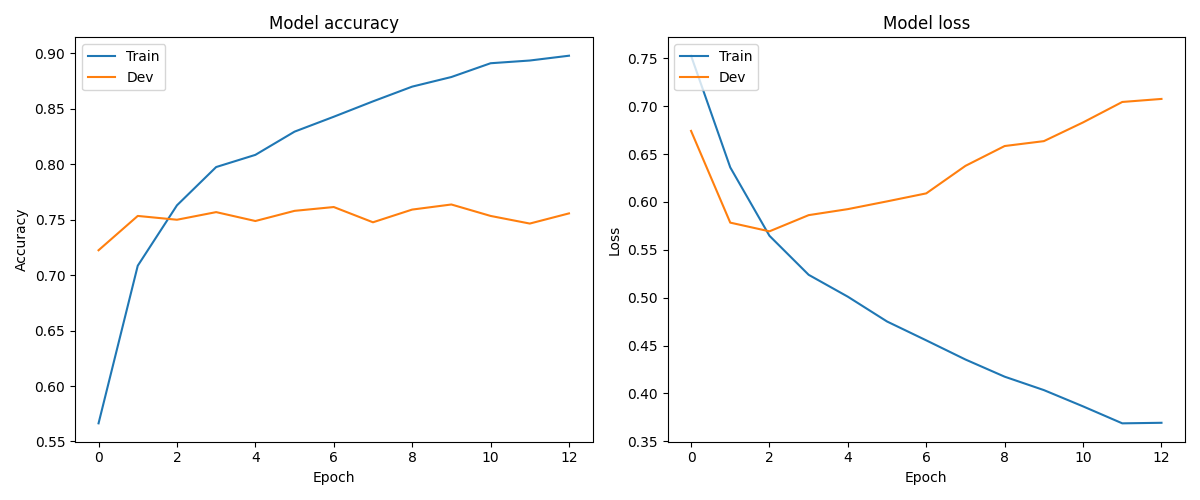
\includegraphics[width=0.8\textwidth]{.img/perceptron1.png}
          \caption{Resultados de la implementación inicial}
        \end{figure}
        \clearpage
      \subsection*{Implementación final}
        \begin{lstlisting}[language=Python, caption=Implementación final del perceptron]
# === Librerías ===

import numpy as np
import tensorflow as tf
from tensorflow.keras import regularizers
from tensorflow.keras.callbacks import EarlyStopping
from tensorflow.keras.layers import Dropout
from tensorflow.keras.preprocessing import text
from sklearn.utils import shuffle
import re
import pandas as pd
import matplotlib.pyplot as plt
import time

# === Funciones ===

def load_data(path):
    training_set = load_sst_data(path+'train.txt')
    dev_set = load_sst_data(path+'dev.txt')
    test_set = load_sst_data(path+'test.txt')
    return training_set, dev_set, test_set

def load_sst_data(path,
                  easy_label_map={0:0, 1:0, 2:None, 3:1, 4:1}):
    data = []
    with open(path) as f:
        for i, line in enumerate(f):
            example = {}
            example['label'] = easy_label_map[int(line[1])]
            if example['label'] is None:
                continue

            # Strip out the parse information and the phrase labels---we don't need those here
            text = re.sub(r'\s*(\(\d)|(\))\s*', '', line)
            example['text'] = text[1:]
            data.append(example)
    data = pd.DataFrame(data)
    return data

def preprocess_data(training_set, dev_set, test_set):
    # Shuffle dataset
    training_set = shuffle(training_set)
    dev_set = shuffle(dev_set)

    test_set = shuffle(test_set)

    # Obtain text and label vectors, and tokenize the text
    train_texts = training_set.text
    train_labels = training_set.label

    dev_texts = dev_set.text
    dev_labels = dev_set.label

    test_texts = test_set.text
    test_labels = test_set.label

    # Create a tokenize that takes the 1000 most common words
    tokenizer = text.Tokenizer(num_words=1000)

    # Build the word index (dictionary)
    tokenizer.fit_on_texts(train_texts) # Create word index using only training part

    # Vectorize texts into one-hot encoding representations
    x_train = tokenizer.texts_to_matrix(train_texts, mode='binary')
    x_dev = tokenizer.texts_to_matrix(dev_texts, mode='binary')
    x_test = tokenizer.texts_to_matrix(test_texts, mode='binary')

    y_train = train_labels
    y_dev = dev_labels
    y_test = test_labels
    
    return x_train, y_train, x_dev, y_dev, x_test, y_test

def create_model(input_shape, hidden_units, dropout_rate, l1_lambda, l2_lambda):
    model = tf.keras.models.Sequential()
    model.add(tf.keras.layers.Input(shape=(input_shape,)))
    for units in hidden_units:
        model.add(tf.keras.layers.Dense(units, activation='relu', kernel_regularizer=regularizers.l1_l2(l1=l1_lambda, l2=l2_lambda)))
        model.add(Dropout(dropout_rate))
    model.add(tf.keras.layers.Dense(1, activation='sigmoid'))
    return model

def train_model(model, x_train, y_train, x_dev, y_dev, epochs, batch_size):
    model.compile(optimizer='adam', loss='binary_crossentropy', metrics=['accuracy'])
    early_stopping = EarlyStopping(monitor='val_accuracy', patience=3)
    history = model.fit(x_train, y_train, epochs=epochs, batch_size=batch_size, validation_data=(x_dev, y_dev), callbacks=[early_stopping])
    return model, history

def evaluate_model(model, x_test, y_test):
    loss, accuracy = model.evaluate(x_test, y_test)
    return loss, accuracy

def run_experiment(hidden_units, dropout_rate, l1_lambda, l2_lambda, epochs, batch_size):
    model = create_model(x_train.shape[1], hidden_units, dropout_rate, l1_lambda, l2_lambda)
    model, history = train_model(model, x_train, y_train, x_dev, y_dev, epochs, batch_size)
    loss, accuracy = evaluate_model(model, x_test, y_test)
    return loss, accuracy, history

def draw_results(history):
    fig, (ax1, ax2) = plt.subplots(1, 2, figsize=(12, 5))
    
    ax1.plot(history.history['accuracy'])
    ax1.plot(history.history['val_accuracy'])
    ax1.set_title('Model accuracy')
    ax1.set_ylabel('Accuracy')
    ax1.set_xlabel('Epoch')
    ax1.legend(['Train', 'Dev'], loc='upper left')
    
    ax2.plot(history.history['loss'])
    ax2.plot(history.history['val_loss'])
    ax2.set_title('Model loss')
    ax2.set_ylabel('Loss')
    ax2.set_xlabel('Epoch')
    ax2.legend(['Train', 'Dev'], loc='upper left')
    
    plt.tight_layout()
    plt.show()

# === Main ===

if __name__ == "__main__":
    # Iniciamos una seed tanto para numpy como para tensorflow
    np.random.seed(1)
    tf.random.set_seed(2)
    
    # Cargamos los datos
    training_set, dev_set, test_set = load_data('Data/')
    # Preprocesamos los datos
    x_train, y_train, x_dev, y_dev, x_test, y_test = preprocess_data(training_set, dev_set, test_set)
    
    # Definimos los hiperparámetros
    hidden_units_list = [[50, 50], [100, 50], [100, 100]]
    dropout_rate_list = [0.3, 0.5, 0.7]
    l1_lambda_list = [0.001, 0.01, 0.1]
    l2_lambda_list = [0.001, 0.01, 0.1]
    batch_size_list = [32, 64, 128]
    epochs = 100

    best_accuracy = 0
    best_params = None
    best_history = None

    startTime = time.time()
    for hidden_units in hidden_units_list:
        for dropout_rate in dropout_rate_list:
            for l1_lambda in l1_lambda_list:
                for l2_lambda in l2_lambda_list:
                    for batch_size in batch_size_list:
                        print(f"Training with hidden_units={hidden_units}, dropout_rate={dropout_rate}, l1_lambda={l1_lambda}, l2_lambda={l2_lambda}, batch_size={batch_size}")
                        loss, accuracy, history = run_experiment(hidden_units, dropout_rate, l1_lambda, l2_lambda, epochs, batch_size)
                        if accuracy > best_accuracy:
                            best_accuracy = accuracy
                            best_loss = loss
                            best_params = (hidden_units, dropout_rate, l1_lambda, l2_lambda, batch_size)
                            best_history = history
    print(f"Training time: {time.time()-startTime}")

    print(f"Best accuracy & lost: {best_accuracy} & {best_loss} with parameters: hidden_units={best_params[0]}, dropout_rate={best_params[1]}, l1_lambda={best_params[2]} l2_lambda={best_params[3]}, batch_size={best_params[4]}")
    
    # Dibujamos los resultados del mejor modelo
    draw_results(best_history)
    
        \end{lstlisting}
        \begin{figure}[H]
          \centering
          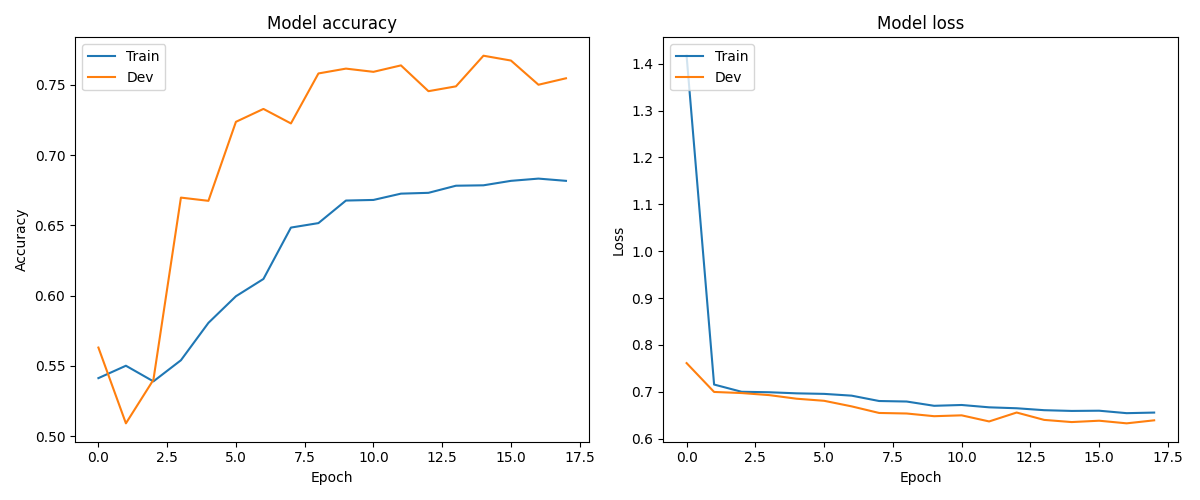
\includegraphics[width=0.8\textwidth]{.img/perceptron2.png}
          \caption{Resultados de la implementación final}
        \end{figure}
        \clearpage
      \subsection*{Conclusines}
        \paragraph*{La primera implementación:}
        {
          Para llevar a cabo esta implementación, hemos utilizado un perceptron con dos capas ocultas de 50 neuronas cada una.
          Ademas, para evitar el sobreajuste, hemos utilizado regularización L2, Dropout y Early stopping.
          
          \begin{itemize}
            \item \textbf{Regularización L2:} La regularización L2 añade un término de penalización a la función de pérdida del modelo para limitar la complejidad de los parámetros del modelo y fomentar generalización.
            \item \textbf{Dropout:} Dropout es una técnica que consiste en desactivar aleatoriamente un porcentaje de las neuronas de la red en cada iteración. De esta forma, se evita que la red se sobreajuste a los datos de entrenamiento.
            \item \textbf{Early stopping:} Early stopping es una técnica que consiste en detener el entrenamiento de la red cuando el error en el conjunto de validación comienza a aumentar. De esta forma, se evita el sobreajuste.
          \end{itemize}

          En la primera implementación la precisión del conjunto de entrenamiento sigue aumentando y parece estabilizarse alrededor de 0.9 hacia el final de las épocas. Esto podria sugerir que el modelo está aprendiendo bien los patrones del conjunto de entrenamiento.
          No obstante, la curva con el conjunto de desarrollo se estanca en 0.75 y no aumenta. Esto podría ser indicativo de un problema de sobreajuste, ya que el modelo sigue mejorando en el entrenamiento, pero no tanto en el conjunto de validación.\\

          De igual forma, la pérdida del conjunto de entrenamiento disminuye constantemente y de manera significativa, lo que es un comportamiento esperado para un modelo que está aprendiendo correctamente.
          Sin embargo, la pérdida del conjunto de validación disminuye inicialmente, pero luego comienza a aumentar después de unas pocas épocas. Esto es un indicativo claro de sobreajuste, ya que el modelo comienza a ajustarse demasiado a los datos de entrenamiento y pierde capacidad de generalización.
        }
        \paragraph*{La segunda implementación:}
        {
          En esta implementación hemos añadido regularización L1 y hemos hecho un barrido de hiperparametros para encontrar la mejor configuración.
          Hemos probado con diferentes configuraciones de capas ocultas, porcentaje de dropout, lambdas de regularización y tamaño de batch para ver cual daba un mejor resultado de precisión.

          \begin{itemize}
            \item \textbf{Regularización L1:} añaden un término de penalización a la función de pérdida del modelo para limitar la complejidad de los parámetros del modelo y fomentar generalización.
          \end{itemize}

          La diferencia entre la regularización L1 y L2 es que L1 tiende a hacer que los pesos de las neuronas sean 0, mientras que L2 tiende a hacer que los pesos sean pequeños pero no 0.
          Esto hace que L1 sea bueno en modelos donde muchas de las características son irrelevantes, ya que las pone a 0, mientras que L2 es bueno en modelos donde todas las características son relevantes en su mayoria.
          Tambien existe ElasticNet que es una combinación de L1 y L2.\\

          En esta implementacion, tanto los datos de entrenamiento como los de validación han crecido de manera constante y pareja, lo que indica que el modelo está aprendiendo correctamente y no está sobreajustando.
          No obstante, posiblemente debido a un tamaño de datos pequeños, la precisión no ha sido muy alta.\\

          Respecto a las metricas de perdida, ambas han disminuido de manera constante y pareja, lo que indica que el modelo está aprendiendo correctamente y no está sobreajustando como si pasaba en la primera implementación.
        }

  \chapter{Resultados}
    \section{Autograder}
      \begin{lstlisting}
Question q1
===========
*** q1) check_regression
Your final loss is: 0.018517
*** PASS: check_regression

### Question q1: 6/6 ###

Question q2
===========
*** q2) check_digit_classification
Your final test set accuracy is: 97.140000%
*** PASS: check_digit_classification

### Question q2: 6/6 ###

Finished at 8:39:09

Provisional grades
==================
Question q1: 6/6
Question q2: 6/6
------------------
Total: 12/12
    \end{lstlisting}
\end{document}